%% LyX 1.6.5 created this file.  For more info, see http://www.lyx.org/.
%% Do not edit unless you really know what you are doing.
\documentclass[english]{article}
\usepackage[T1]{fontenc}
\usepackage[latin9]{inputenc}
\usepackage[letterpaper]{geometry}
\geometry{verbose,tmargin=1in,bmargin=1in,lmargin=1in,rmargin=1in}
\usepackage{amstext}
\usepackage[authoryear]{natbib}
\usepackage{graphicx}
\usepackage{subcaption}

%%%%%%%%%%%%%%%%%%%%%%%%%%%%%%
%% New commands
\newcommand{\tgf}{TGF-$\beta$}

\usepackage{babel}

\begin{document}

\title{Supplementary Content}

\maketitle
\section{Quality control graphs}

%\begin{figure}
%	\centering
%	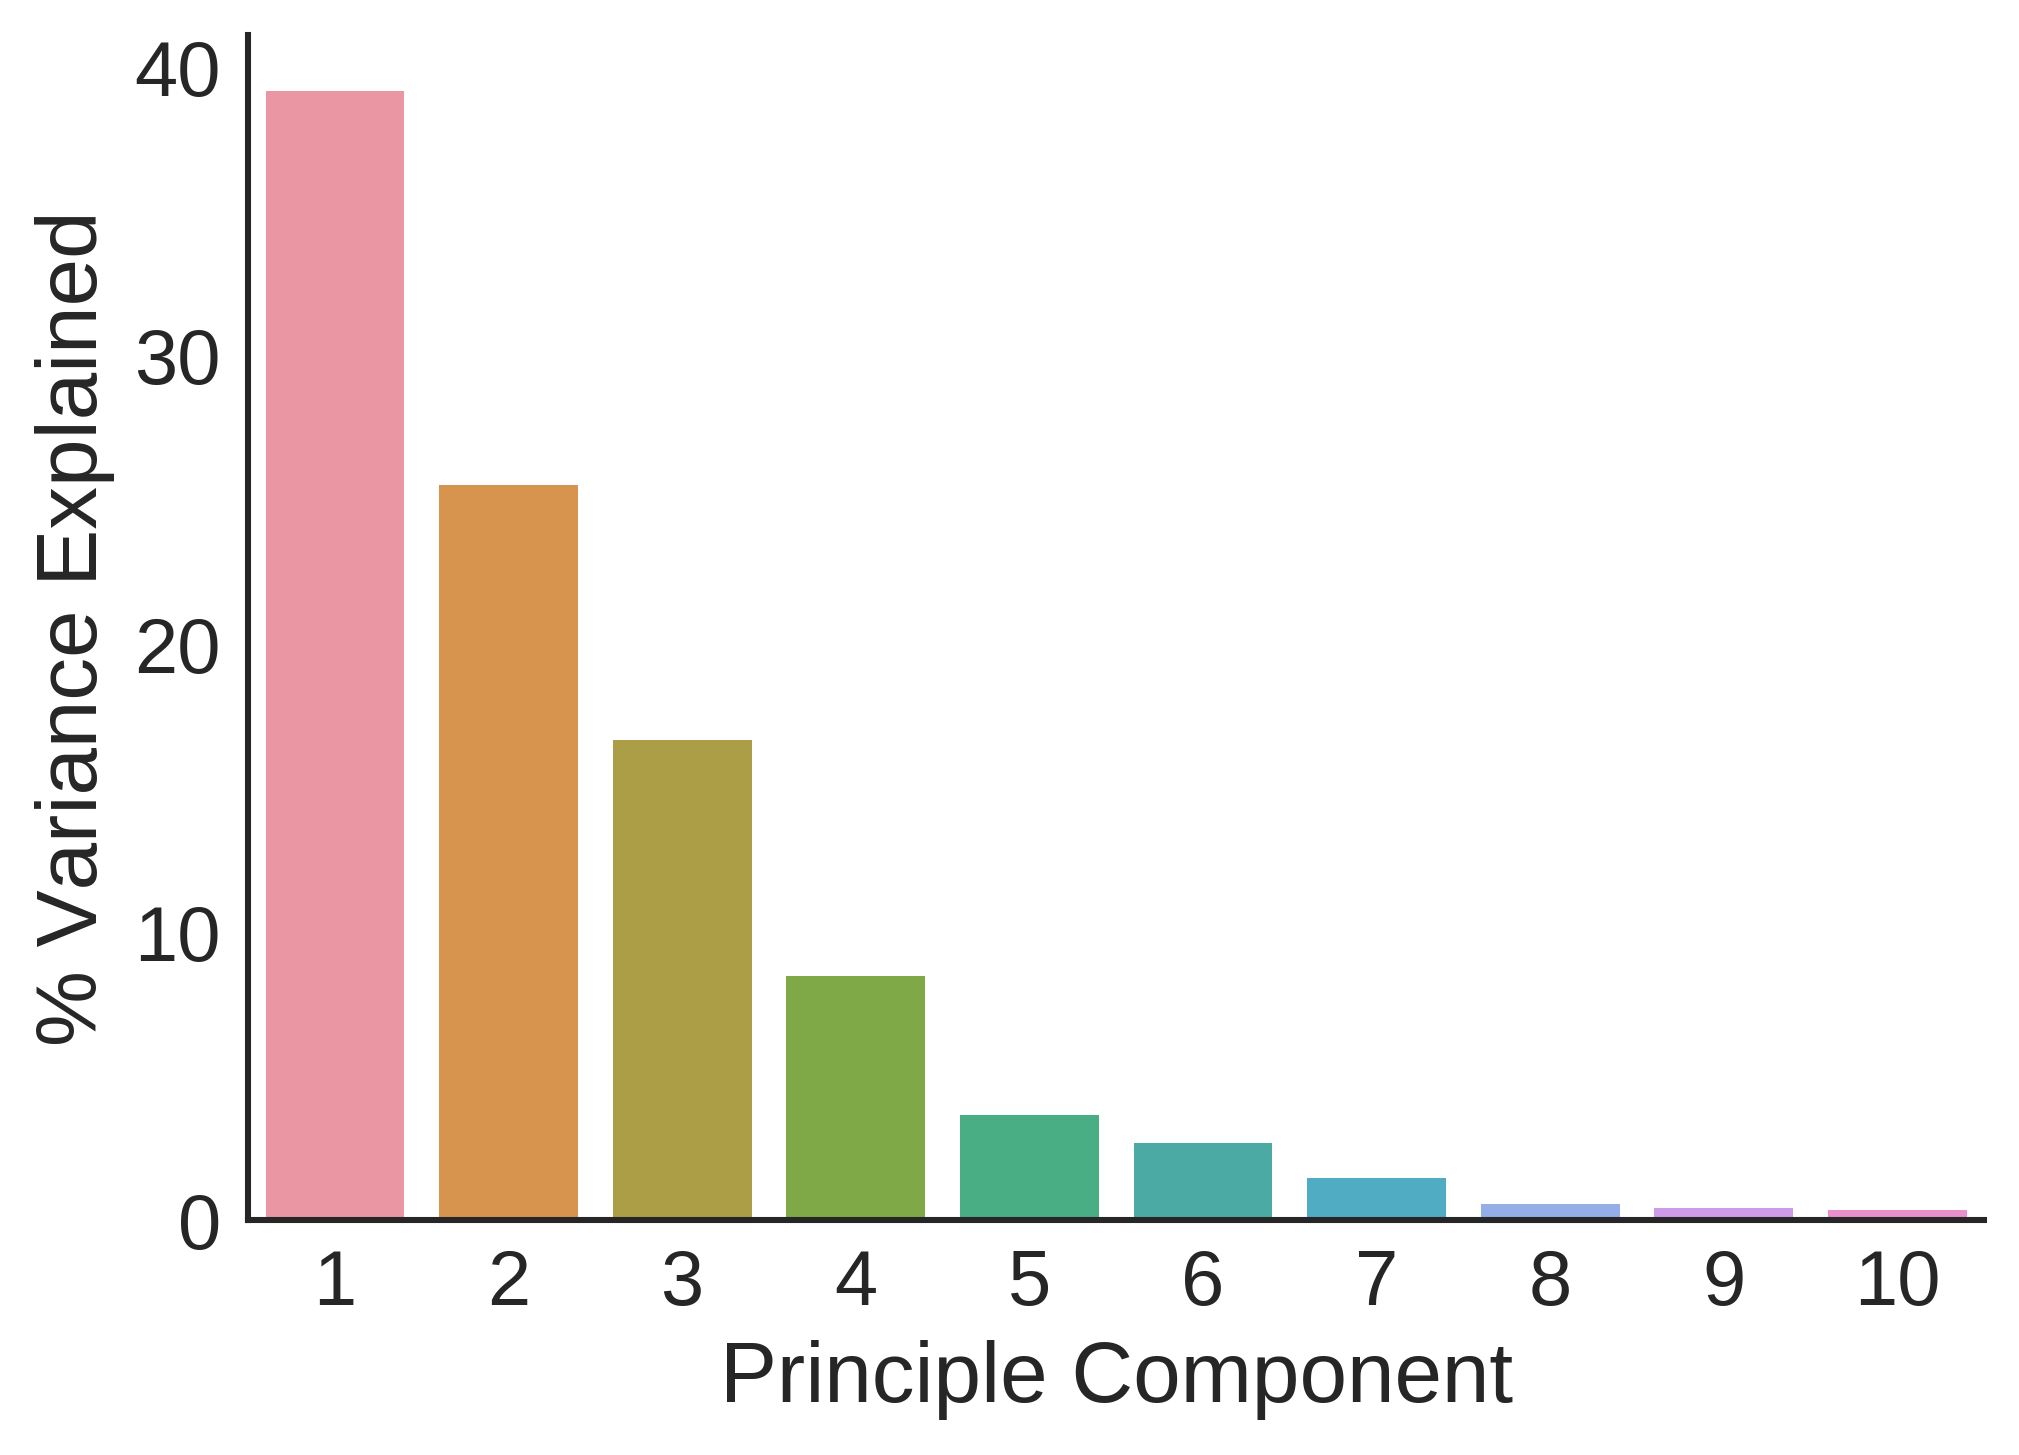
\includegraphics[width=\linewidth]{img/qc/pca_scree}
%	\caption{Plot showing the percent of variance explained for the first 10 principal components.}
%	\label{sfig:qc:scree}
%\end{figure}
%
%\begin{figure}
%	\centering
%	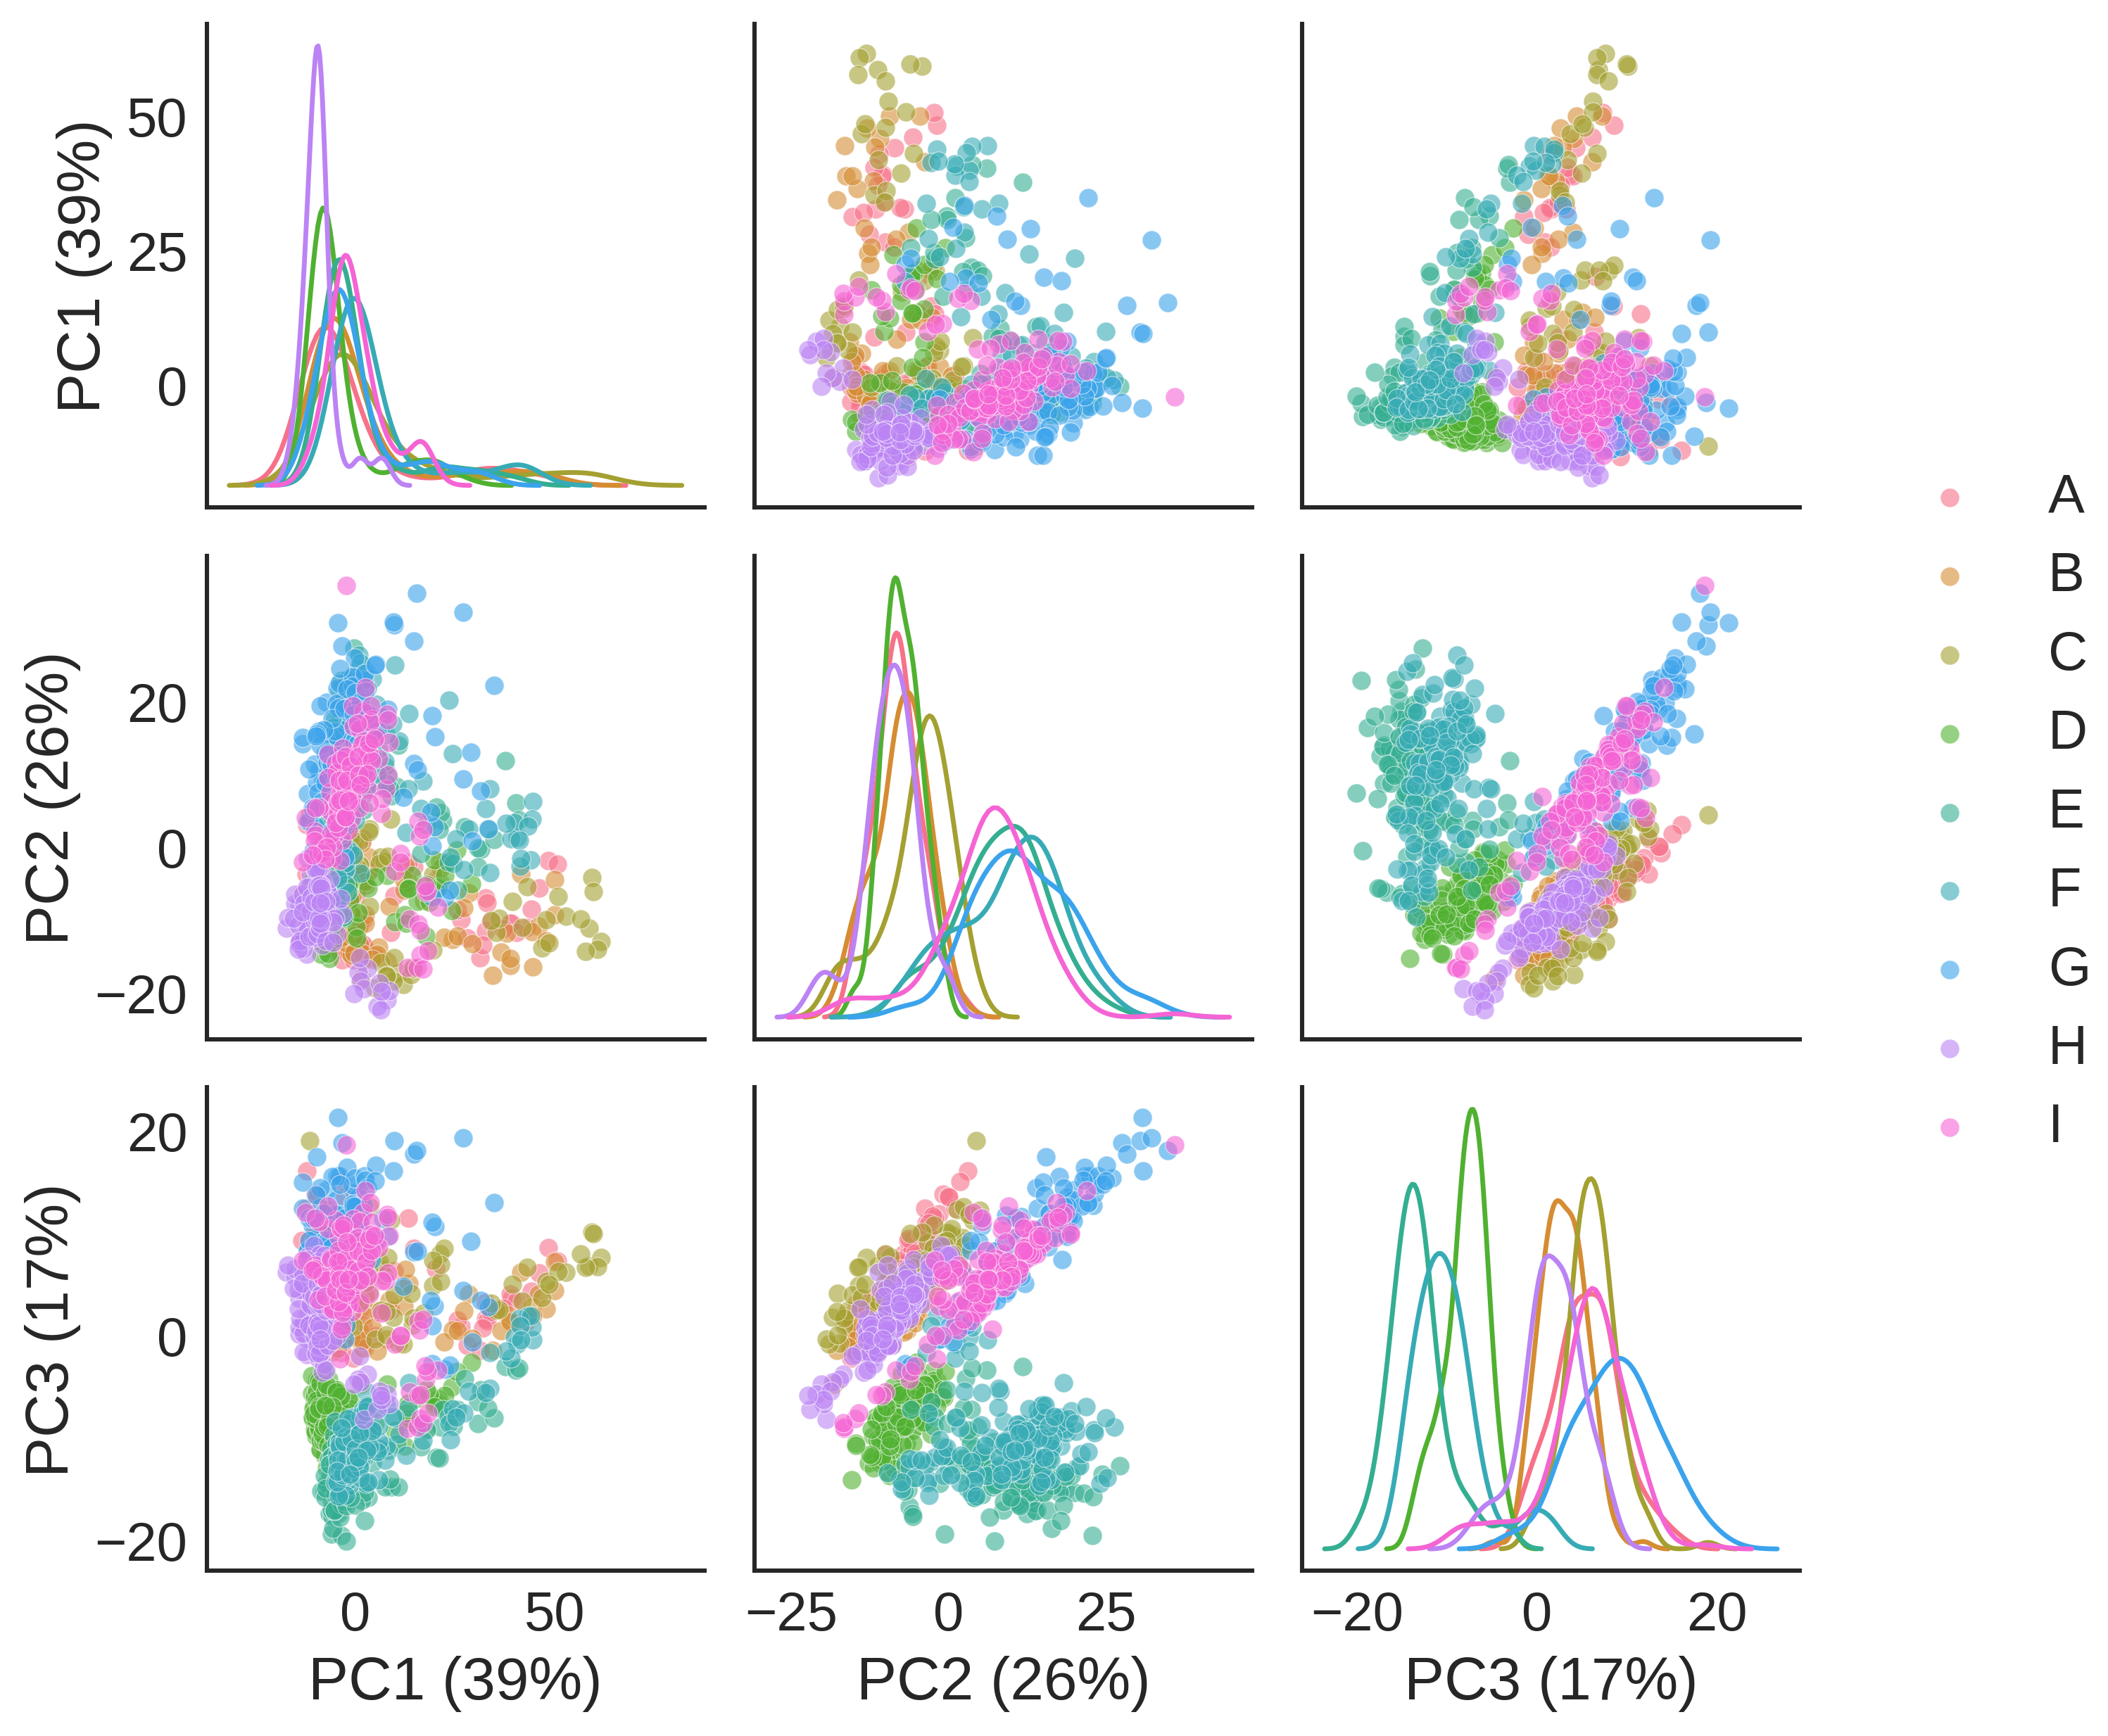
\includegraphics[width=\textwidth]{img/qc/cell_id}
%	\caption{Scatter matrix of first three principle components coloured by cell id.}
%	\label{fig:qc:cell_id}
%\end{figure}
%
%\begin{figure}
%	\centering
%	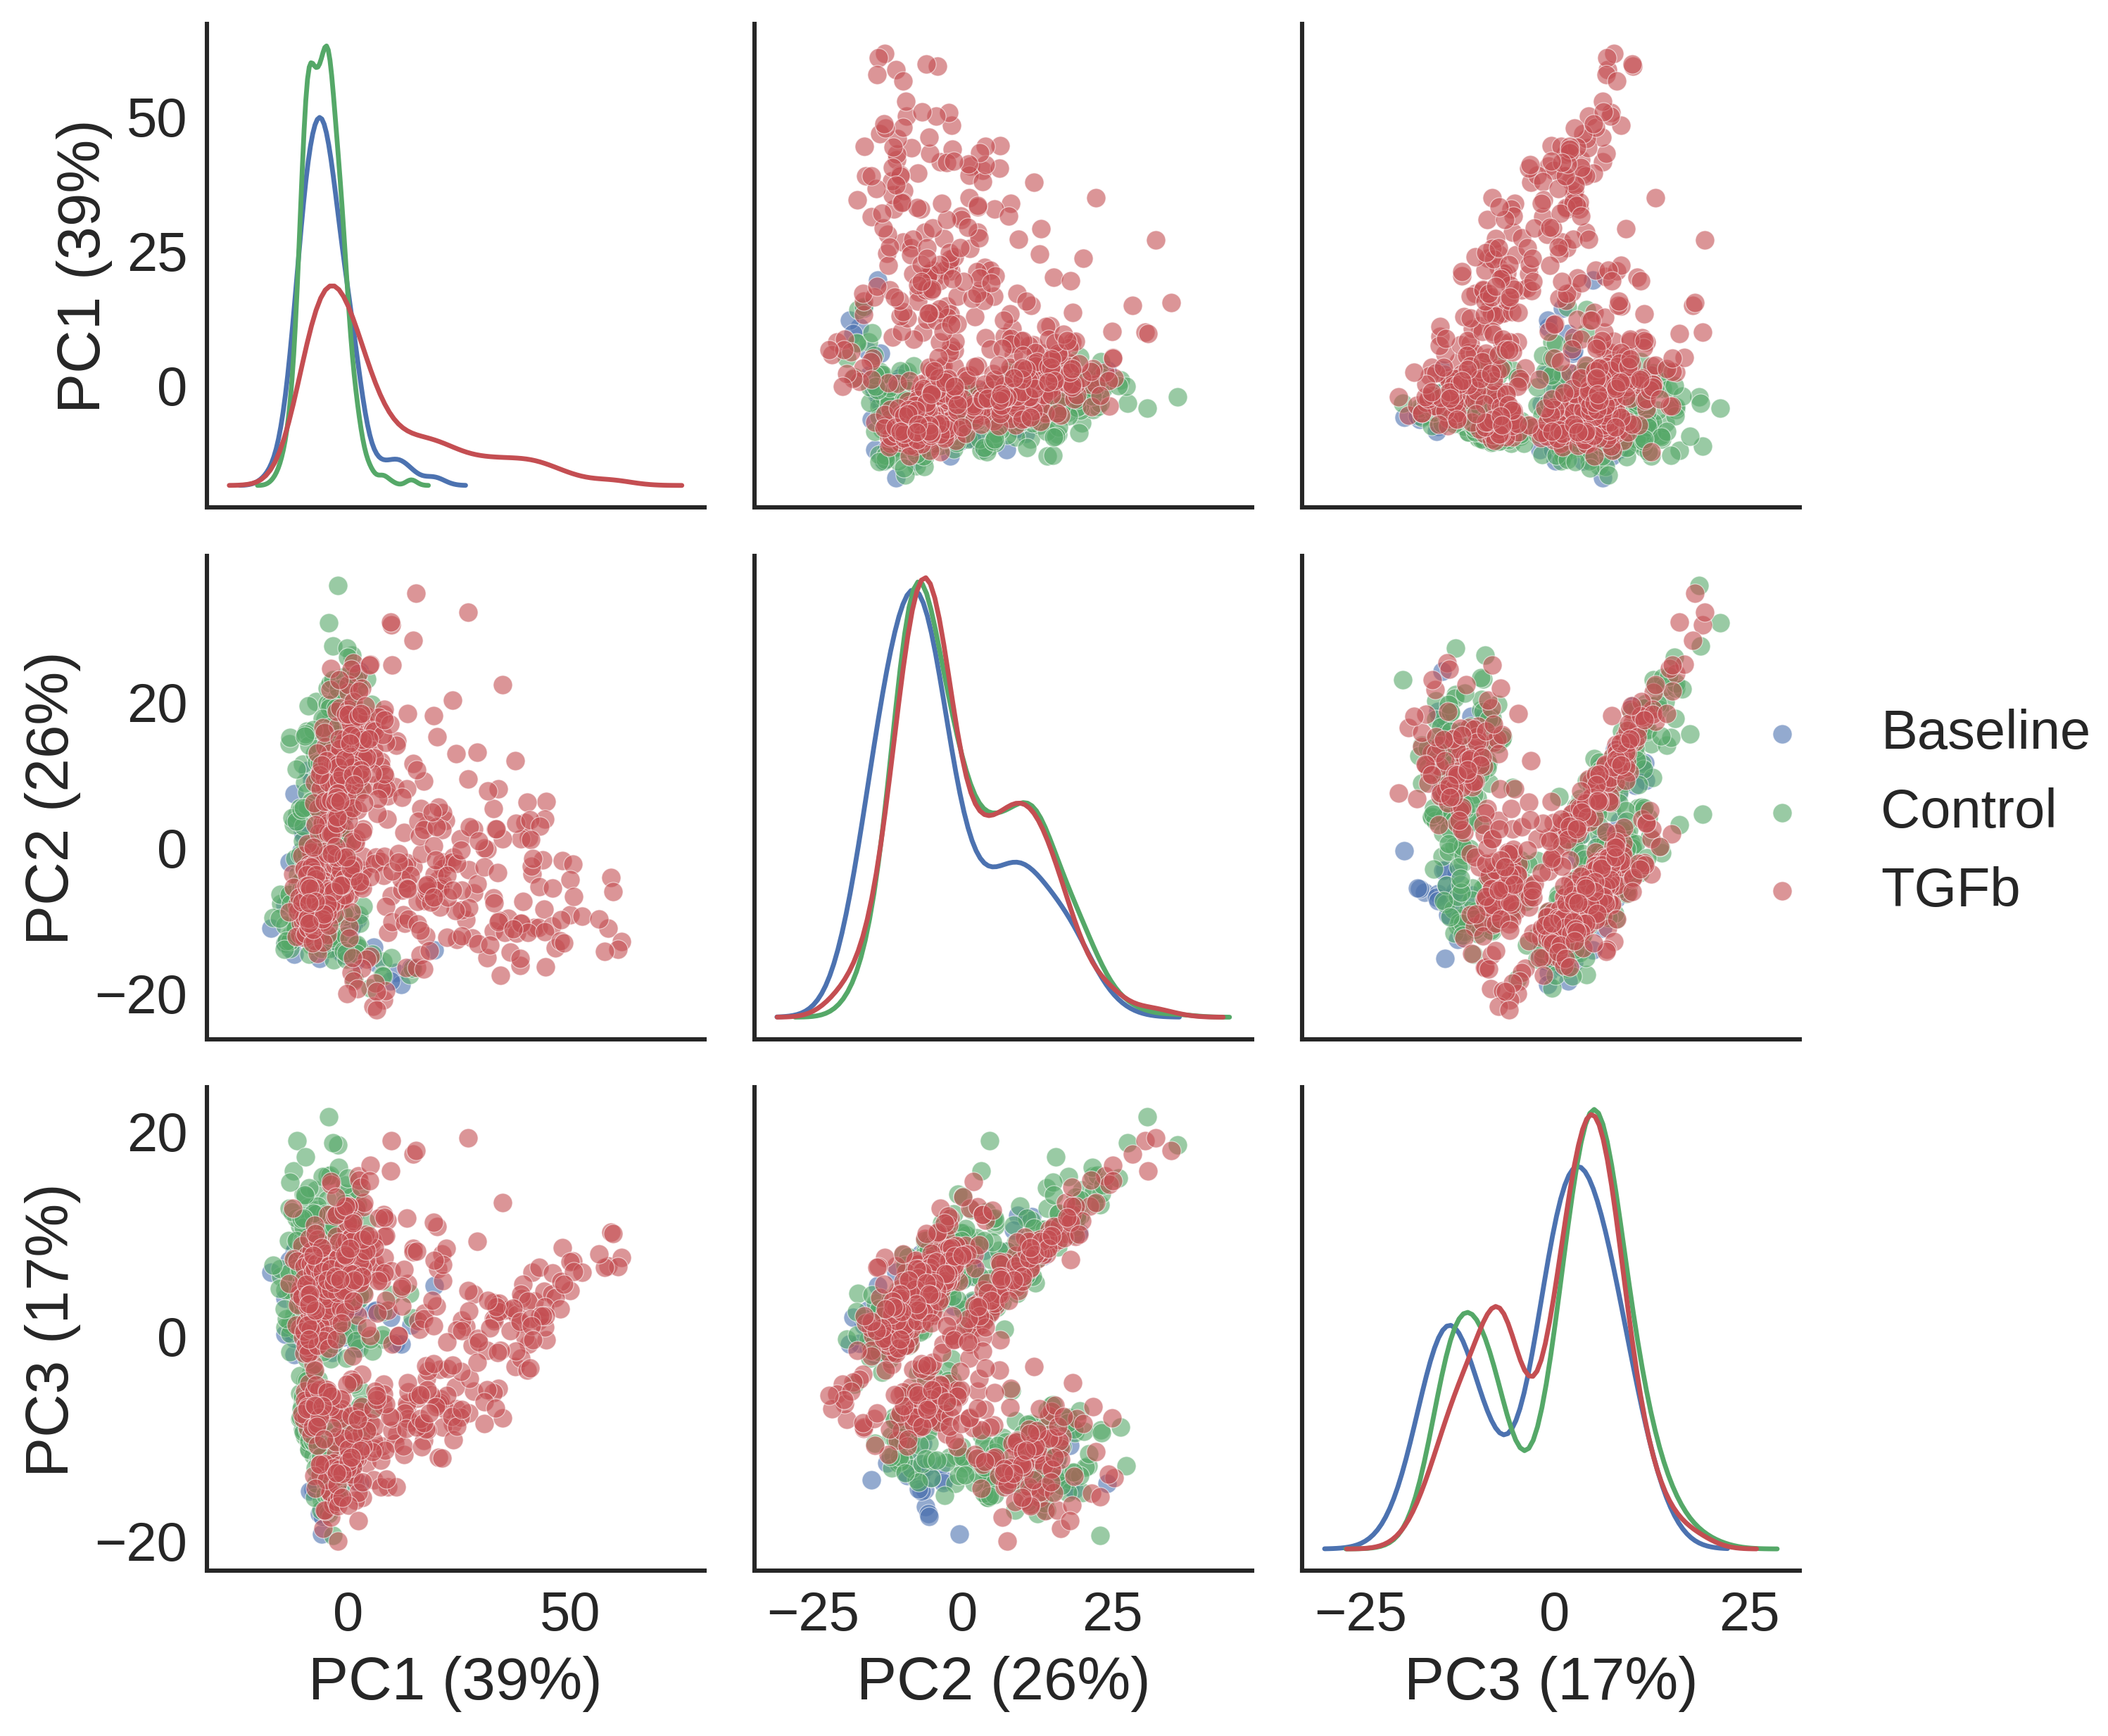
\includegraphics[width=\textwidth]{img/qc/treatment}
%	\caption{Scatter matrix of first three principle components coloured by treatment.}
%	\label{fig:qc:treatment}
%\end{figure}
%
%\begin{figure}
%	\centering
%	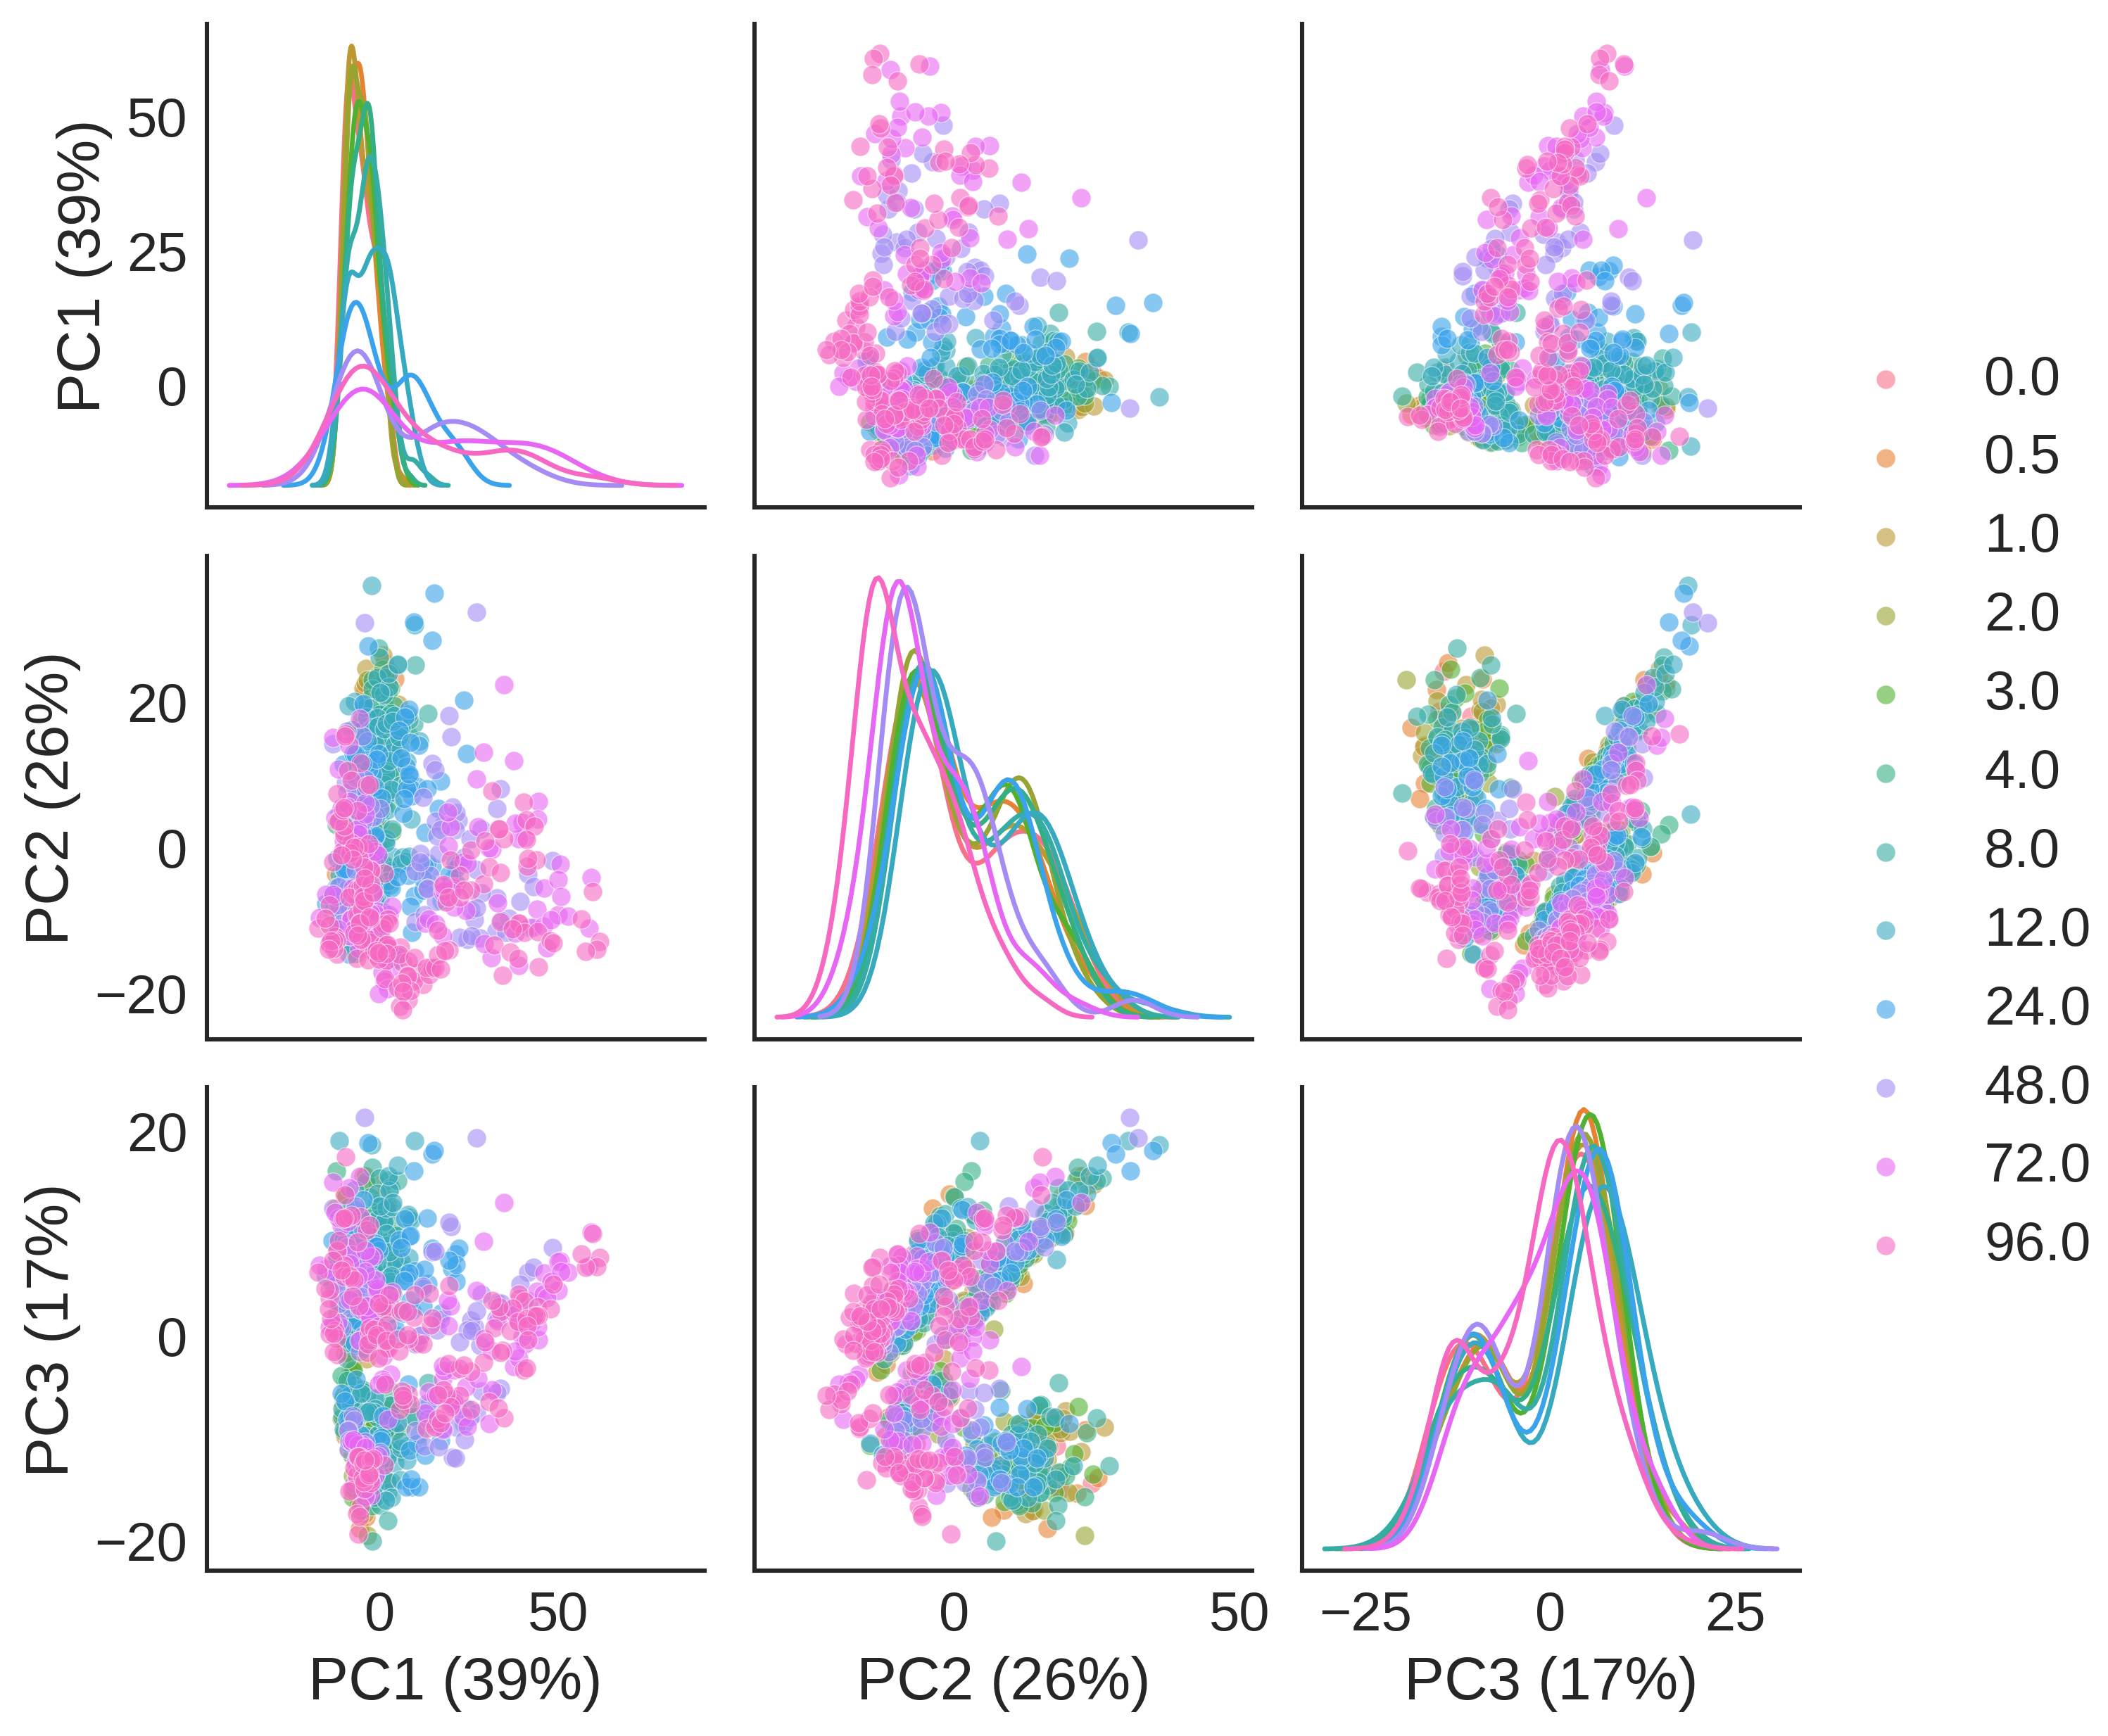
\includegraphics[width=\textwidth]{img/qc/time_point}
%	\caption{Scatter matrix of first three principle components coloured by time point.}
%	\label{fig:qc:time_point}
%\end{figure}
%
%\begin{figure}
%	\centering
%	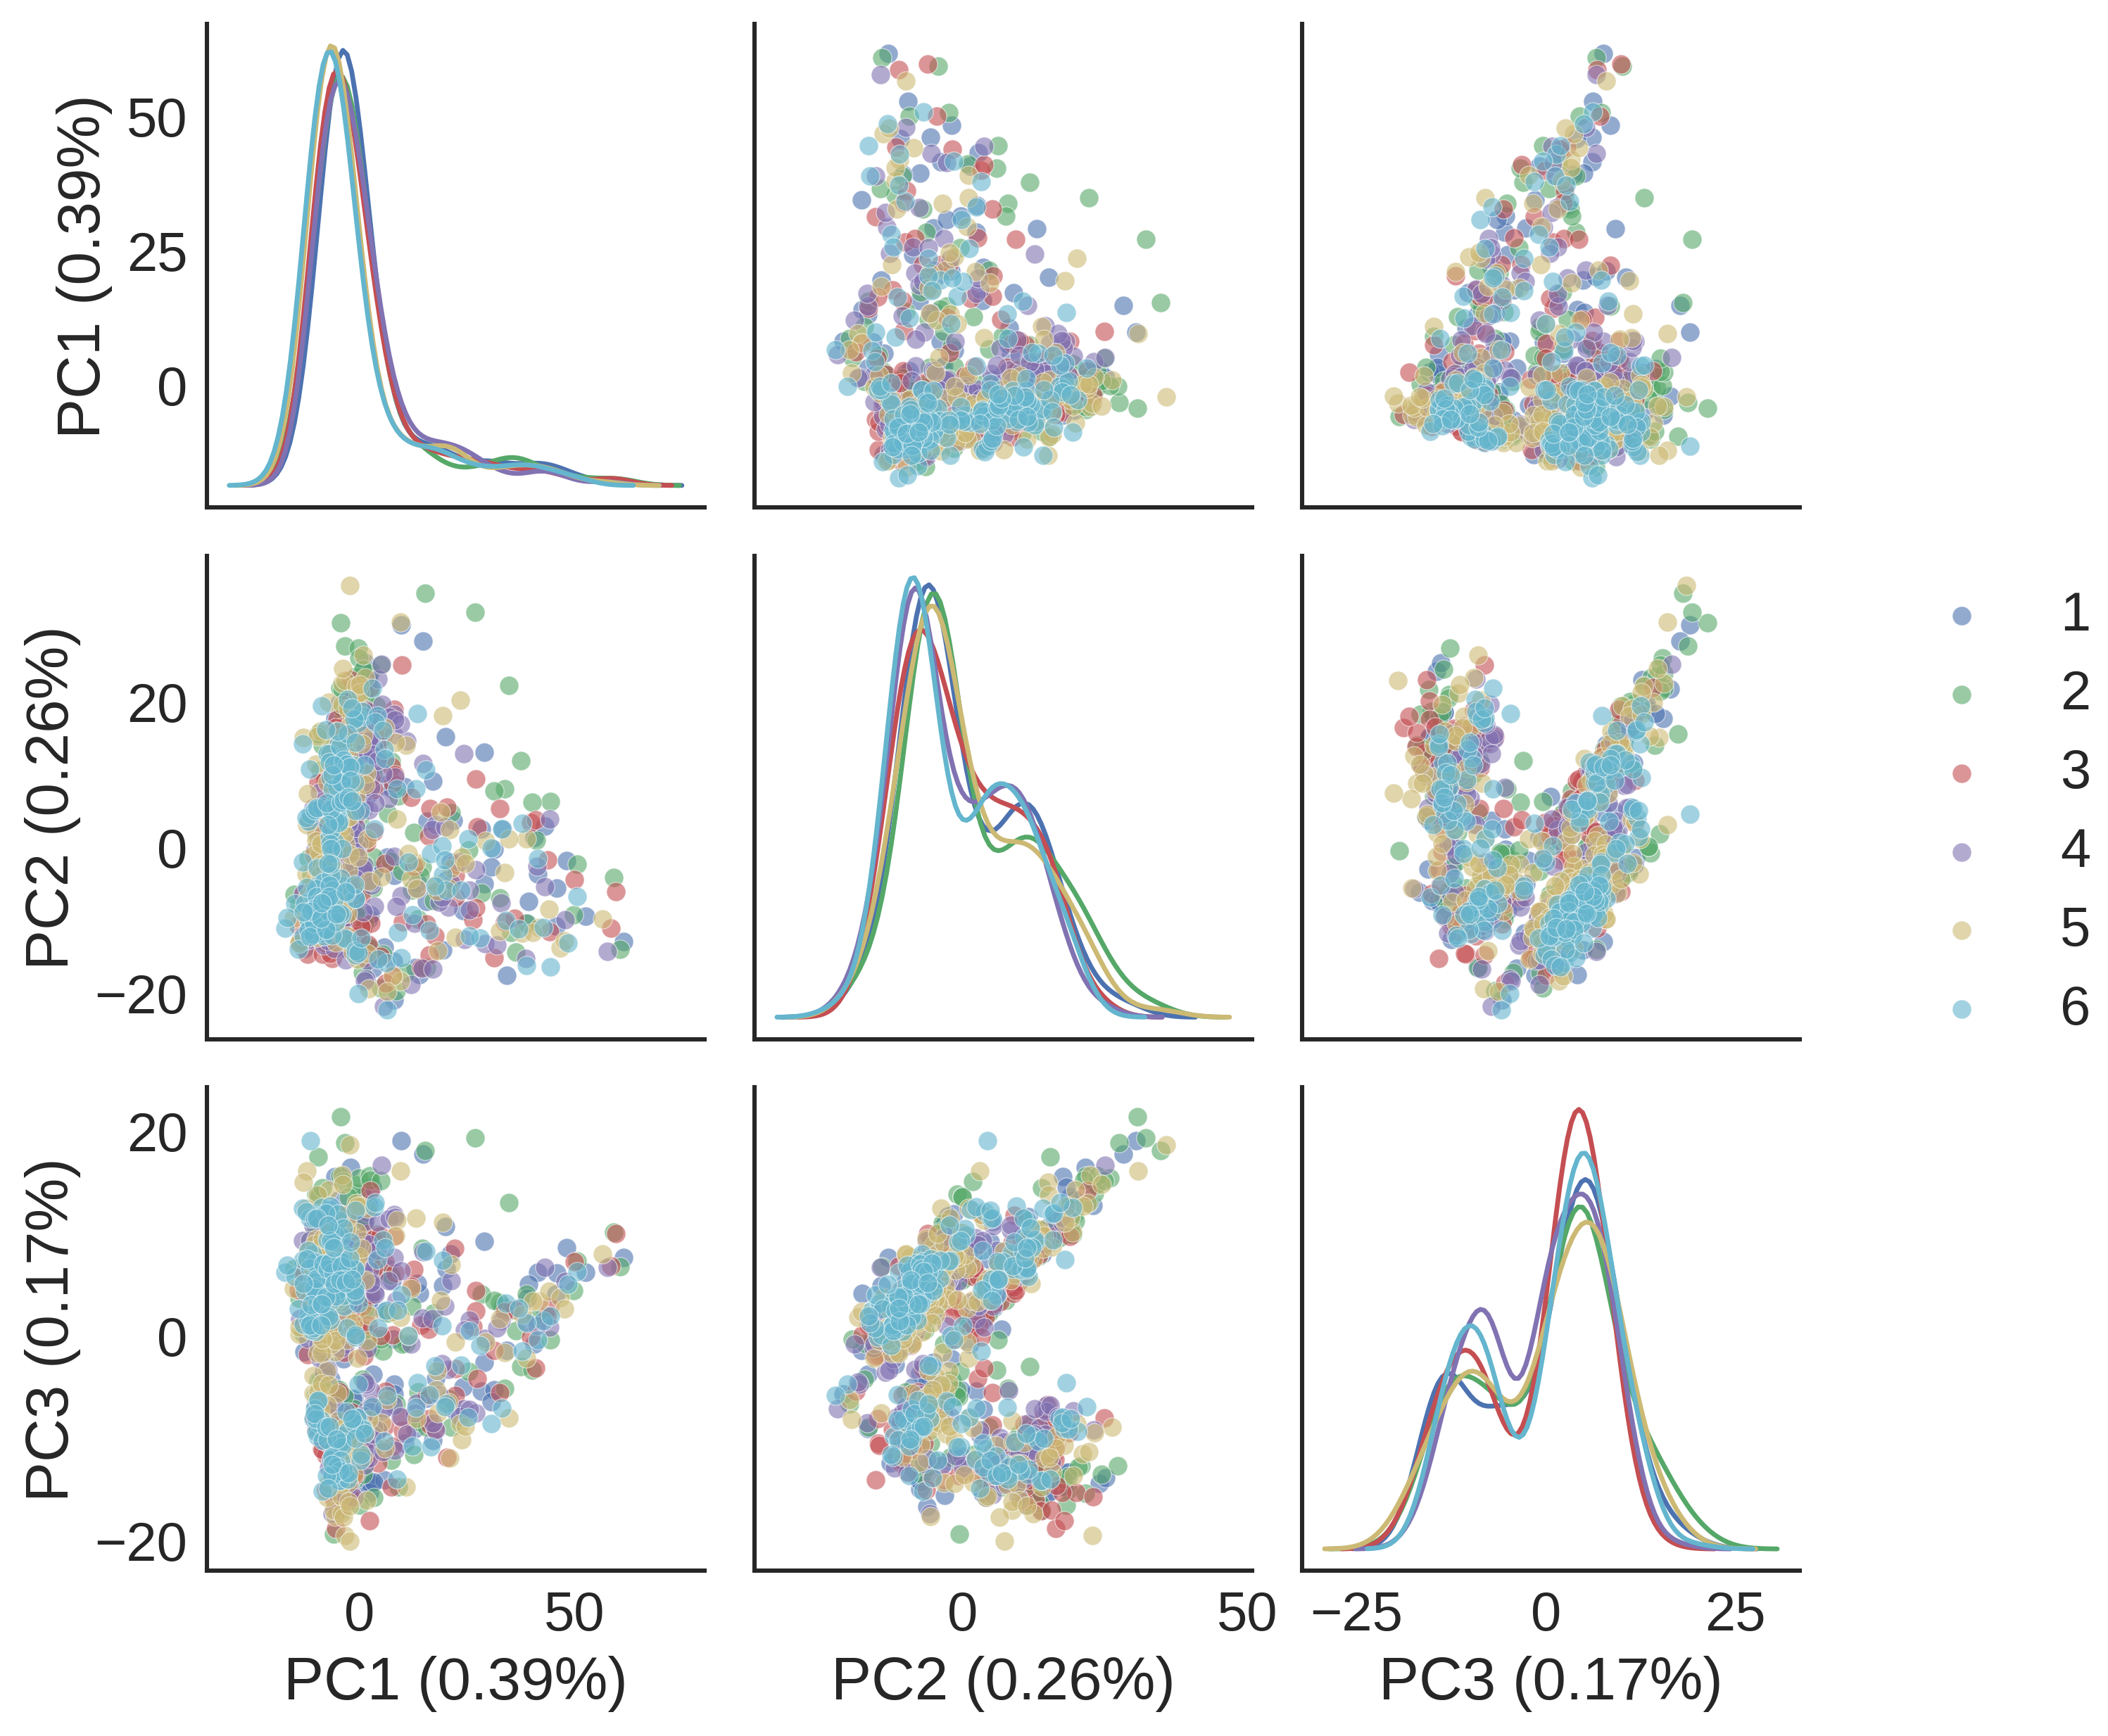
\includegraphics[width=\textwidth]{img/qc/replicate}
%	\caption{Scatter matrix of first three principle components coloured by replicate.}
%	\label{fig:qc:replicate}
%\end{figure}
%\bibliographystyle{msb}
%\bibliography{sample}

\end{document}
